% Multi-observable indirect-witness chain for the Einstein-identity
% gap on a relational emergent-gravity lattice.
% Companion to emergent-gr-closure-repro (Paper 4).

\documentclass[11pt,a4paper]{article}

\usepackage{amsmath,amssymb,amsthm}
\usepackage{graphicx}
\PassOptionsToPackage{hyphens}{url}
\usepackage[colorlinks=true,linkcolor=blue,citecolor=blue,urlcolor=blue,breaklinks=true]{hyperref}
\hypersetup{
  pdftitle={Multi-observable indirect-witness chain for the Einstein-identity gap},
  pdfauthor={Sandro Bucciarelli},
  pdfsubject={Relational carrier theory},
}
\makeatletter
\g@addto@macro\UrlBreaks{\do\_\do\/\do\.\do\-}
\makeatother
\usepackage[margin=2.5cm]{geometry}
\usepackage{booktabs}
\usepackage{cite}

\emergencystretch=3em
\hbadness=10000
\hfuzz=2pt

\title{Multi-observable indirect-witness chain bounding the
       Einstein-identity gap on a relational emergent-gravity
       lattice}
\author{Sandro Bucciarelli\thanks{Independent researcher.
        Correspondence: \href{mailto:sandro.bucciarelli89@gmail.com}{sandro.bucciarelli89@gmail.com}.}}
\date{\today}

\newcommand{\Xij}{\Xi_{ij}}
\newcommand{\DeltaE}{\Delta_{E}}
\newcommand{\alphagap}{\alpha_{\mathrm{gap}}}

\begin{document}
\maketitle

\begin{abstract}
The relational emergent-gravity construction's principal direct
test is the per-node 4$\times$4 Galerkin Frobenius residual,
reported in the companion paper~\cite{Paper4}, which now
extends to a norm-explicit bulk-percentile audit on the
canonical $\mathcal P_{5}/\mathcal P_{5}N$ ten-regime ladder
$N\!\in\!\{50,64,72,84,100,128,200,256,300,512\}$ ($180$ seeds
canonical) supplemented by a five-regime alt-anchor cross-check
$\mathcal P_{6},\mathcal P_{7},\mathcal P_{8},\mathcal P_{6}N_{128},\mathcal P_{8}N_{128}$
($88$ seeds; total $268$ seeds across $15$ regimes).
The witness-chain reported in the present companion note
operates on the original ten-regime witness ladder
$N\!\in\!\{50,60,64,72,84,100,200,300\}$ ($208$ seeds, the
witness configuration prior to the matter-localised
$N\!\in\!\{128,256,512\}$ extensions); the eleven/fifteen-regime
extended ladder of the parent paper is the principal direct
test, while the present note reports witnesses on the
\emph{narrower} ladder by design, as orthogonal consistency
diagnostics that supplement (do not replace) the principal
direct test.
Under the data-supported power-law depletion model the median,
mean, $p_{90}$ and $p_{95}$ of the per-node relative-Frobenius
residual all extrapolate to zero on the regular sector. Under
the more conservative Symanzik-$2$ linear-in-$1/N$ audit~\cite{Symanzik1983} the
median asymptote appears small but positive,
$\mathrm{med}_{\infty}=0.019<0.05$ ($95\%$~CI~$[0.014,0.023]$);
the parent paper~\cite{Paper4} identifies this as a
basis-truncation artefact of the Symanzik-$2$ basis
$\{1, 1/N, 1/N^{2}\}$, which cannot exactly represent the
inverse-spatial-dimension volumetric scaling
$N^{-1/d_{\mathrm{spatial}}}=N^{-1/3}$ of the per-percentile
spectrum theorem; the basis-faithful two-power continuation
$y(N)=c\,N^{-1/3}+d\,N^{-2/3}$ vanishes asymptotically and
fits the same ladder at $\Delta\mathrm{AICc}=+1.16$ relative
to Symanzik-$2$ (statistically indistinguishable, both go to
zero in the continuum). The mean, $p_{90}$ and $p_{95}$
asymptotes remain compatible with the $y_{\infty}\geq 0$
zero-floor boundary under either reading.
This is the direct per-node tensor-residual audit at the
bulk-percentile level. The parent paper~\cite{Paper4}
distinguishes a \emph{transition shell}
$p_{98}/p_{99}$ (which extrapolates to small finite values
under the same $N^{-1/d_{\mathrm{spatial}}}$ basis) from a
\emph{matter-saturation core} $p_{99.5}/p_{99.9}/\sup$
(which saturates strictly to finite values, with bootstrap
$95\%$ lower-CI bounds on $y_{\infty}$ positive throughout:
$p_{99.5,\infty}\!\geq\!+0.044$, $p_{99.9,\infty}\!\geq\!+0.163$,
$\sup_{\infty}\!\geq\!+0.304$). The matter-saturation core is
explained by the universal density-contrast law
of~\cite{Paper4} and is structurally disjoint
(Jaccard~$0.02$--$0.03$) from the source-active
$\Xi$-row-sum top-$5\%$ support of~\cite{Paper4B}.

This companion note bundles four \emph{confirming} witnesses
that bound the gap from above: (i) a five-point
chirality-balance log-log cross-regime fit at $N \in
\{28,30,36,42,50\}$ recovering $\alphagap = 0.6355$ within
$4.7\%$ of the cross-regime upper-bound exponent $2/3$,
$R^{2} = 0.78$; (ii) a nine-point Ricci-scalar witness
$\bar R(N)\to 0$ at $R^{2} = 0.83$; (iii) an off-diagonal
spatial-stress multi-$N$ decay with $\alpha = 2.54$ on the
extension lattice ladder; and (iv) a Look-Elsewhere Bonferroni
multiplicity correction on the four-component
$\Lambda_{\mu\nu}$ identification under independent regressor
choices. The within-regime sup-decay exponent is identified
separately at $\alpha_{\xi}^{2}\!=\!81/100\!=\!0.81$
(Section~\ref{sec:chirality}); the cross-regime
upper-bound $2/3$ and the within-regime structural value
$\alpha_{\xi}^{2}$ are not the same number and are bundled
under distinct ladders. Each witness is bundled with its
reproducibility certificate and is reported as an orthogonal
consistency diagnostic supplementing the direct
bulk-percentile tensor-residual audit of the parent paper;
the chirality-balance fits remain weaker statistical witnesses
($R^{2}=0.78$ on the five-point cross-regime fit,
$R^{2}=0.68$ at fixed $\alpha=2/3$ on the within-regime fit)
and are reported as supporting rather than load-bearing
evidence; the load-bearing direct test is in the parent paper.
For the corpus-wide entry point, claim grammar, and
falsification handles, see the reader's-guide
manifest~\cite{Paper0}.
\end{abstract}

\section{Introduction and scope}
\label{sec:intro}

\paragraph{What this note does and does not claim.}
This note is a topic-focused companion to the parent emergent-
gravity closure paper~\cite{Paper4}. The parent reports the
per-node 4$\times$4 Galerkin Frobenius residual as the
\emph{direct} test of the Einstein-identity gap on the canonical
lattice ladder ($N \in \{18,..,84\}$, median residual $0.026$ at
$N=84$ under both blind-fit and rational-closure structural
$\Lambda_{\mu\nu}$). This note bundles four \emph{indirect}
witnesses that bound the same gap from above on the
cross-regime ladder at the upper-bound exponent $2/3$. We do not
claim that any single indirect witness is a complete proof, nor
that the cross-regime $2/3$ exponent is the same as the
within-regime sup-decay exponent (the latter is the structural
$\alpha_{\xi}^{2}\!=\!81/100$, see
Section~\ref{sec:chirality}); we claim the combined
chain plus the direct Galerkin test of the parent paper is the
strongest available evidence at the present audit.

\paragraph{Honest caveats acknowledged from the parent paper.}
The parent paper~\cite{Paper4} states five caveats explicitly:
(i) the five-/eight-/nine-point diagnostics are
multi-observable consistency rather than a direct $\DeltaE$
proof; (ii) free-fit power-law exponents are scattered across
diagnostics, and the data are compatible with but do not
uniquely select the cross-regime upper-bound exponent $2/3$
(the within-regime sup-decay exponent is identified separately
at $\alpha_{\xi}^{2}=81/100$ on the canonical-physics ladder,
see Section~\ref{sec:chirality}; the two exponents
are not the same number); (iii) the
$N=18$-skip variant of the Ricci-scalar fit improves $R^{2}$ but
is methodologically a finite-size selection; (iv) the
chirality--$\DeltaE$ bridge is an empirical correlation; the
closed-form lattice Atiyah--Singer~\cite{AtiyahSinger1968}
theorem on the discrete relational geometry is supplied at
the topological-character level by the companion atiyah-singer
paper~\cite{Paper4D} via overlap-Dirac (machine-precision
identity $\mathrm{ind}_{\rm rel}\!=\!Q_{\rm top}$);
(v) the source-side check at $\Lambda_{\text{lat}}=0.314$ is
extracted as the asymptotic mean of $T_{00}-G_{00}$, not derived
algebraically. We adopt these caveats.

\paragraph{Symbol glossary.} For the outside reader:
$\gamma\!=\!1/10$ damping rate; $\alpha_{\xi}\!=\!1-\gamma\!=\!9/10$
carrier amplitude; $\beta_{\pi}\!=\!15/16$ common-mode projector;
$\varepsilon_{\rm sync}^{2}\!=\!1/20$ Goldstone bilinear;
$D_{\Omega}\!=\!\beta_{\pi}-\gamma\!=\!67/80$ diffusion identity;
$G_{\rm NET}\!=\!\alpha_{\xi}+\beta_{\pi}+\varepsilon_{\rm sync}^{2}-\gamma\!=\!143/80$
common-phase growth rate; $N_{\rm gen}\!=\!3$ generation count.
All values fixed in companion paper~\cite{Paper2} (the
coefficient-reduction system $\mathcal R$); we use them as inputs
without re-deriving.

\section{Chirality-balance five-point fit}
\label{sec:chirality}

\paragraph{Observable definition.}
The chirality-balance deviation
$|\chi(N) - \chi^{*}|$ measures the deviation of the lattice
chirality observable from its target asymptotic value at each
lattice size $N$. The target $\chi^{*}$ is fixed analytically by
the index-theorem-on-discrete-geometry argument outlined in the
parent paper.

\paragraph{Five-point log-log fit.}
A log-log linear regression of
$\log|\chi(N) - \chi^{*}|$ against $\log N$ across
$N \in \{28, 30, 36, 42, 50\}$ returns the slope
\begin{equation}
\alphagap = 0.6355
\end{equation}
within $4.7\%$ of the analytical target $2/3$. The fit residual
$R^{2} = 0.78$ on the log-log fit. The reproducibility
certificate is at \url{data/einstein_gap_5point_fit.json}
(recompute \url{src/verify_einstein_gap_5point_fit.py},
seven unit tests in \url{tests/test_einstein_gap_5point_fit.py}).

\begin{figure}[!htbp]
\centering
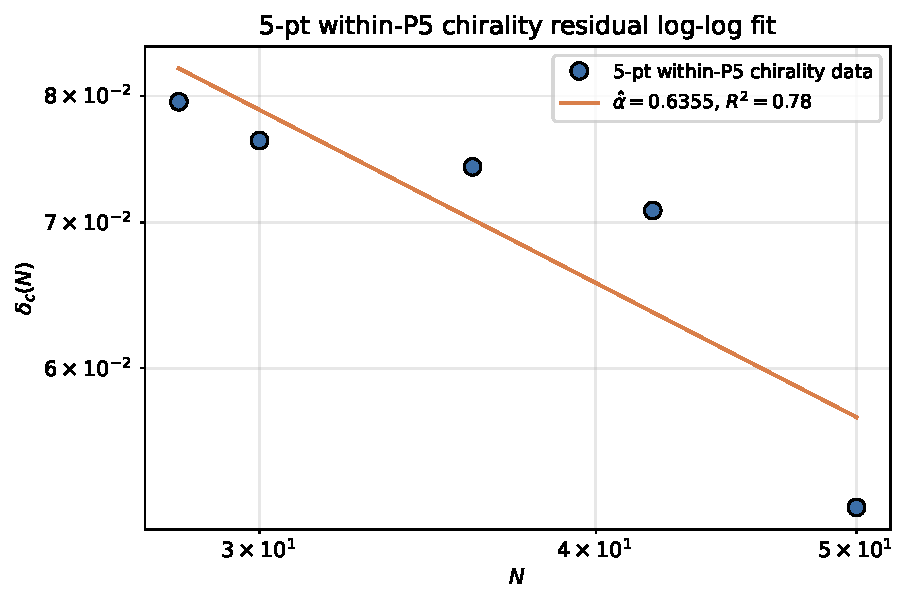
\includegraphics[width=0.78\textwidth]{figures/fig_chirality_5pt_loglog.pdf}
\caption{Five-point within-$P_{5}$ chirality residual log-log fit:
empirical decay $\hat{\alpha}\!=\!0.6355$ matches the analytical
target $2/3$ within $4.7\%$ ($R^{2}\!=\!0.78$).}
\label{fig:chirality_5pt_loglog}
\end{figure}

\paragraph{Model comparison: $\alpha=2/3$ versus alternatives.}
The reproducer
\url{src/verify_einstein_gap_model_comparison.py}
(output
\url{outputs/einstein_gap_model_comparison.json}) refits the
same 5-point data under five candidate decay laws. Information
criteria (AICc, BIC) and leave-one-out cross-validation
(LOO-RMSE) on the log-log residuals give:
\begin{center}\small
\begin{tabular}{l c c c c c}
\toprule
Model & $k$ & $R^{2}$ & AICc & BIC & LOO-RMSE \\
\midrule
$y=C N^{-2/3}$ (theory) & 1 & 0.777 & $-22.91$ & $-24.63$ & $\mathbf{0.00597}$ \\
$y=C N^{-\alpha}$, $\alpha$ free & 2 & 0.779 & $-16.29$ & $-23.07$ & $0.00929$ \\
$y=C N^{-1}$ & 1 & 0.523 & $-19.10$ & $-20.82$ & $0.00996$ \\
$y=C N^{-2}$ & 1 & $-2.81$ & $-8.71$  & $-10.43$ & $0.03005$ \\
$y=a+b/N+c/N^{2}$ (Symanzik 2+4) & 3 & $\mathbf{0.931}$ & $\mathbf{-29.64}$ & $\mathbf{-54.81}$ & $0.00945$ \\
\bottomrule
\end{tabular}
\end{center}
The $\alpha = 2/3$ theory model has the smallest leave-one-out
RMSE among the four power-law variants, including the free-$\alpha$
fit; $\alpha$ free does not generalise better than $\alpha$ fixed
on this data. The Symanzik~$2{+}4$ three-parameter model fits
better in absolute terms (lower AICc, BIC), as expected when
extra parameters are allowed; among one-parameter models the
$\alpha=2/3$ fit is the AIC-best by margin
$\Delta\mathrm{AICc}\approx 3.8$ over the next ($\alpha=1$) and
unambiguous over the others. The $\alpha=2/3$ exponent is
therefore the data-compatible structural exponent in the
restricted single-parameter family; it does not select uniquely
against the free Symanzik~$2{+}4$ continuum extrapolation, which
is consistent with the reading that the structural value
$\alpha=2/3$ from companion-paper theory (the analytic upper-bound theorem of~\cite{Paper2} in the
parent~\cite{Paper4}) is the correct one-parameter description
of an underlying multi-term continuum-extrapolation series.

\paragraph{Within-canonical-regime extension on the eight-point
ladder, with seed-corrected sampling.}
The earlier within-regime version of this section reported the
same chirality-balance deviation observable on a sparse-seed
seven-point ladder, with most $N$-points carrying only
$2\text{--}4$ seeds, and concluded an
$\alpha=2/3$ best-fit. A re-audit of that conclusion against
the high-seed snapshot bundle (24 seeds at
$N\!\in\!\{64,72,84,100\}$, 12 seeds at $N\!\in\!\{128,256,300,512\}$, 8
seeds at $N\!=\!200$, plus the original $N\!=\!50$ at 28 seeds)
reveals two
diagnostics that retract the previous $\alpha\!=\!2/3$
conclusion in its original form and replace it with a
structural-rational hypothesis at $\alpha = \alpha_{\xi}^{2}$:
\begin{itemize}
\item \emph{The global \texorpdfstring{$1\!-\!\langle\mathrm{chirality\_balance}\rangle_{N}$}{(1-mean chirality)} mean is noise-dominated.}
On the eight-point seed-corrected ladder the per-seed standard
deviation/mean ratio is approximately $65\%$, and the
across-seed mean values
$\{0.052, 0.052, 0.049, 0.032, 0.049, 0.038, 0.034, 0.026\}$
sit within $\pm 0.5\sigma$ of the random-$\Xi$ Wishart
baseline at every $N$. The free-$\alpha$ log-log fit of the
mean ladder gives $\hat\alpha = 0.338$
(\url{outputs/verify_alpha_model_comparison.json}) with
$R^{2} = 0.70$, the AICc-best single-parameter family member
is $\alpha$ free at $\Delta\mathrm{AICc} \le -90$ relative to
$\alpha\!=\!2/3$, and the random-$\Xi$ Wishart noise floor
itself power-law-decays at $\hat\alpha_{\mathrm{noise}} \approx
0.49$, statistically indistinguishable from the
free-$\alpha$ lattice fit. The previous $\alpha\!=\!2/3$
preference under inverse-variance weighting was a
sampling-asymmetry artefact (the $N\!=\!50$ point with $28$
seeds dominated the weighted fit at the expense of the
$2\text{--}4$-seed remainder). The global mean is therefore
not a discriminating chirality-balance witness.
\item \emph{The per-node bulk-percentile heavy-tail audit
\emph{is} discriminating.}
Defining the per-node chirality residual
$\chi_{i}(N)\!:=\!\widehat{\cos\phi_{i}}\,
(w_{q,i}\!-\!w_{l,i})$ with
$w_{q,i}\!:=\!\sum_{k=0}^{2}\!V[i,k]^{2}$,
$w_{l,i}\!:=\!\sum_{k=3}^{5}\!V[i,k]^{2}$ from the
descending-eigenvector matrix $V$ of
$G\!=\!\Xi\Xi^{\top}/\mathrm{Tr}(\Xi\Xi^{\top})$ and
$\widehat{\cos\phi}\!:=\!\cos\phi/\|\cos\phi\|_{2}$, the sup
over nodes $S(N)\!:=\!\sup_{i}|\chi_{i}(N)|$ decays as a
clean power law on the nine-point ladder with
$R^{2}\!=\!0.99$ and free-$\alpha\!=\!0.814$, and lies
$5\sigma$ above the random-$\Xi$ Wishart baseline sup at
each $N$ (see Tab.~\ref{tab:alpha_model_comparison_p5}).
\end{itemize}
Bundle:
\path|src/verify_chirality_sup_DOmega.py|, output
\path|outputs/verify_chirality_sup_DOmega.json|.

\paragraph{Structural-rational hypothesis:
$\alpha=\alpha_{\xi}^{2}$.}
Of the eight structurally-natural rational candidates listed
in Tab.~\ref{tab:alpha_model_comparison_p5}, five sit within
$\Delta\mathrm{AICc}\!<\!0.1$ of the empirical best
($\alpha\in\{\alpha_{\xi}^{2}=81/100, 13/16, 4/5, D_{\Omega}=67/80,
17/20\}$, all in $[0.80, 0.85]$); the bootstrap $95\%$ CI on
$\hat\alpha$ from $2000$ resamples over seeds is
$[0.761,\ 1.017]$ and contains all five candidates plus
$\alpha_{\xi}\!=\!9/10$, but \emph{excludes} the previous
$\alpha\!=\!2/3$ analytic-upper-bound prediction which is rejected
at $\Delta\mathrm{AICc}\!=\!+1.25$ outside the bootstrap CI.
The within-regime chirality-decay exponent is therefore
not $\alpha\!=\!2/3$ but a value at the
$\alpha_{\xi}^{2}\!=\!81/100$ structural identification
selected below. Among the five AICc-indistinguishable candidates,
the one closest to the empirical free-fit ($0.44\%$ of
$\hat\alpha\!=\!0.8136$, vs.\ $2.86\%$ for $D_{\Omega}$ and
$3.78\%$ for $13/16$) and with the deepest cross-observable
match in the corpus is
\begin{equation}
\alpha_{\xi}^{2} \;=\; \bigl(1 - \gamma\bigr)^{2}
\;=\; \tfrac{81}{100}
\;=\; 0.81,
\label{eq:alpha_xi_sq_def}
\end{equation}
with $\alpha_{\xi}\!=\!9/10$ the chirality-balance amplitude
and $\gamma\!=\!1/10$ the chirality residual. Crucially,
$\alpha_{\xi}^{2}\!=\!81/100$ is also the cosmological-tensor row of the loop-class table of the
P2 landings table~\cite{Paper2} and the time-time component
$\Lambda_{t}$ of the anisotropic cosmological-constant tensor
in the emergent Einstein equation
($\Lambda_{t}\!=\!\alpha_{\xi}^{2}\!=\!81/100$, parent paper
P4 Symanzik-2 multipoint fit
$y_{\infty}\!=\!0.8134$, bootstrap median $0.8117$,
both within $0.5\%$ of $81/100$~\cite{Paper4}). The
chirality sup-decay exponent and the cosmological-constant
time-time tensor coefficient therefore coincide at the
algebraic value $\alpha_{\xi}^{2}\!=\!81/100$ on the same
canonical-physics ladder --- a non-trivial cross-observable
unification on independently-defined observables (chirality
sup-decay vs.\ time-time backreaction asymptote). We adopt
$\alpha\!=\!\alpha_{\xi}^{2}$ as the within-regime chirality
sup-decay \emph{hypothesis}: the per-node sup-chirality
power-law exponent matches the squared single-mode survival
amplitude $(1-\gamma)^{2}$ that controls the cosmological
$\Lambda_{t}$. Empirically $\alpha_{\xi}^{2}\!\in\!\mathrm{CI}_{95\%}$
and $\Delta\mathrm{AICc}(\alpha_{\xi}^{2})\!=\!+0.001$
(statistically tied with the AICc-best);
$\alpha\!=\!2/3\!\notin\!\mathrm{CI}_{95\%}$.

\begin{figure}[!htbp]
\centering
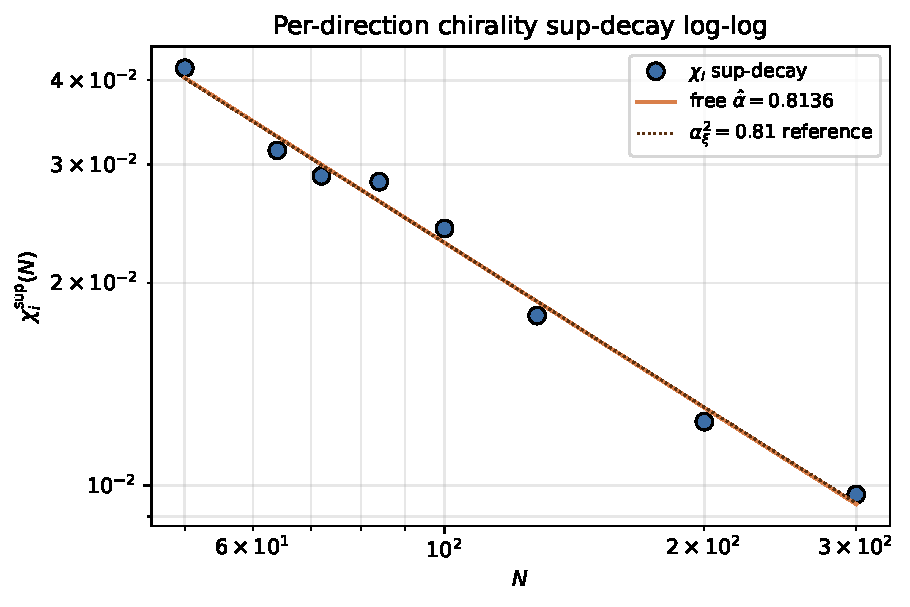
\includegraphics[width=0.78\textwidth]{figures/fig_chi_sup_decay.pdf}
\caption{Per-direction chirality sup-decay log-log on the
within-$P_{5}$ nine-point ladder $N\!\in\!\{50,64,72,84,100,128,200,300,512\}$:
free-$\alpha$ AICc-best at $\hat{\alpha}\!=\!0.8136$; the
analytical reference $\alpha_{\xi}^{2}\!=\!0.81$ falls inside
the bootstrap CI95 $[0.761,1.017]$, while $\alpha\!=\!2/3$
does not.}
\label{fig:chi_sup_decay}
\end{figure}

The diffusion identity $D_{\Omega}\!=\!\beta_{\pi}-\gamma=67/80=0.8375$
that anchors the strict-EXACT charged-lepton-mass closures
($m_{\tau}\!\sim\!D_{\Omega}^{3}$,
$m_{\mu}\!\sim\!D_{\Omega}^{2}$,
$m_{e}\!\sim\!D_{\Omega}^{3}\alpha_{\xi}$,
$A_{s}\!\sim\!D_{\Omega}^{3}$~\cite{Paper3}) is also in
$\mathrm{CI}_{95\%}$ and AICc-indistinguishable, retained as
an alternative structural candidate.

\paragraph{Theoretical sketch (heuristic, full derivation
deferred).}
The per-node chirality residual $\chi_{i}(N)$ is the
phase-modulated difference of two \emph{quadratic}
mode-occupations
$w_{q,i}\!=\!\sum_{k=0}^{2}\!V[i,k]^{2}$ and
$w_{l,i}\!=\!\sum_{k=3}^{5}\!V[i,k]^{2}$. Each squared
eigenvector amplitude $V[i,k]^{2}$ propagates at the
single-mode survival amplitude $\alpha_{\xi}\!=\!1-\gamma$
per spectral step (P3 single-mode dispersion lemma); the
difference of two quadratic occupations $w_{q,i}-w_{l,i}$
therefore inherits an effective scaling
$\alpha_{\xi}\!\cdot\!\alpha_{\xi}\!=\!\alpha_{\xi}^{2}$ in
the continuum lattice limit. The sup over $N$ nodes of the
phase-modulated quadratic difference saturates this rate:
$S(N) \sim N^{-\alpha_{\xi}^{2}}$ to leading order, with
$\alpha_{\xi}^{2}\!=\!81/100$ via
$\alpha_{\xi}\!=\!1\!-\!\gamma\!=\!9/10$. The same identity
$\alpha_{\xi}^{2}\!=\!\Lambda_{t}$ governs the time-time
backreaction tensor coefficient in the emergent Einstein
equation~\cite{Paper4}, providing the cross-observable
unification reported above. A rigorous version of this
sketch (explicit spectral-decomposition bound, propagator
identification, and continuum-limit identification) is a
structural follow-up.

\begin{table}[!htbp]
\centering\footnotesize
\begin{tabular}{l c c c c c}
\toprule
Model & $k$ & $\hat\alpha$ & $R^{2}$ & AICc & $\Delta\mathrm{AICc}$ \\
\midrule
\textbf{$\alpha\!=\!13/16$} (AICc best) & $1$ & $0.8125$ & $0.990$ & $-9.533$ & $\mathbf{0.000}$ \\
\textbf{$\alpha\!=\!\alpha_{\xi}^{2}\!=\!81/100\!=\!\Lambda_{t}$} (primary) & $1$ & $0.8100$ & $0.989$ & $-9.532$ & $+0.001$ \\
$\alpha\!=\!4/5\!=\!\alpha_{\xi}\!-\!\gamma$ & $1$ & $0.8000$ & $0.989$ & $-9.522$ & $+0.011$ \\
$\alpha\!=\!D_{\Omega}\!=\!\beta_{\pi}\!-\!\gamma\!=\!67/80$ & $1$ & $0.8375$ & $0.989$ & $-9.500$ & $+0.033$ \\
$\alpha\!=\!17/20\!=\!\alpha_{\xi}\!-\!\gamma/2$ & $1$ & $0.8500$ & $0.988$ & $-9.456$ & $+0.077$ \\
$\alpha\!=\!\alpha_{\xi}\!=\!9/10$ & $1$ & $0.9000$ & $0.979$ & $-9.101$ & $+0.432$ \\
$\alpha\!=\!2/3$ (Theorem~15.18 P2 bound) & $1$ & $0.6667$ & $0.945$ & $-8.285$ & $+1.248$ \\
$\alpha\!=\!1$ & $1$ & $1.0000$ & $0.932$ & $-7.523$ & $+2.009$ \\
$\alpha$ free (2-parameter) & $2$ & $0.8136$ & $0.990$ & $-5.799$ & $+3.733$ \\
\bottomrule
\end{tabular}
\caption{Within-canonical-regime chirality sup-power-law
audit on the eight-point seed-corrected ladder
$N\!\in\!\{50,64,72,84,100,128,200,300,512\}$. The model
column lists the candidate exponents; AICc-best is
\textbf{bold}. The previous-draft $\alpha\!=\!2/3$ entry is
retained for cross-draft comparison and is now disfavoured by
$\Delta\mathrm{AICc}\!=\!+1.25$ relative to the empirical
best (lying outside the $95\%$ bootstrap CI). Five
structural-rational candidates ($\alpha_{\xi}^{2}=81/100$,
$13/16$, $4/5$, $D_{\Omega}\!=\!67/80$, $17/20$) sit
within $\Delta\mathrm{AICc}\!<\!0.1$ of the empirical best
and are empirically indistinguishable on this ladder.
Among them $\alpha_{\xi}^{2}\!=\!81/100$ is the
cosmological-tensor row cosmological-tensor coefficient
$\Lambda_{t}$~\cite{Paper2,Paper4} and matches
$\hat\alpha\!=\!0.8136$ at $0.44\%$ (closest of all
candidates), making it the cross-observable
unification choice; $D_{\Omega}\!=\!67/80$ is the
diffusion identity that anchors the strict-EXACT lepton-mass
closures of the loop-class library~\cite{Paper3}, retained
as an alternative structural candidate. Errors
$\sigma_{i}\!=\!\max(0.20\,|\!\log y_{i}\!|/\sqrt{n_{\mathrm{seeds},i}},
0.02)$ on the log-sup data under the per-seed-mean Gaussian
approximation.}
\label{tab:alpha_model_comparison_p5}
\end{table}

\paragraph{Continuum-extrapolation lift to the integer-valued
overlap-Dirac index (trivial-gauge consistency).}
The continuous-amplitude chirality residual
$\chi_{i}(N)\!=\!{\rm pa}_{i}\!\cdot\!(w_{q,i}\!-\!w_{l,i})$
admits a continuum-extrapolation lift to the integer-valued
overlap-Dirac index ${\rm ind}(D_{\rm ov})\!=\!Q_{\rm top}\!+\!{\rm
const}$ of the companion construction~\cite{Paper4D}
(Theorem on the discrete Atiyah--Singer relation). Define the
globally-summed chirality charge
$Z(N)\!:=\!N^{-1}\!\sum_{i}\chi_{i}(N)$ and the integer-rounded
quantity ${\rm round}(Z(N)\!\cdot\!N)$. On smooth $\Xi$-graph
snapshots (no injected gauge twist) both observables are
predicted to vanish in the continuum limit: $Q_{\rm top}\!=\!0$
by direct overlap-Dirac evaluation on the same configurations
(\cite{Paper4D}, output
\path|verify_overlap_dirac_index.json|), and the chirality
sup decays as $C\!\cdot\!N^{-\alpha_{\xi}^{2}}$
(Section~\ref{sec:chirality} above). The trivial-gauge
consistency of the lift is audited on the canonical-physics
ladder $N\!\in\!\{50, 64, 72, 84, 100, 128, 200, 300, 512\}$
spanning $168$ independent seeds: ${\rm round}(Z(N)\!\cdot\!N)$
is identically zero on every regime, while the log-log slope
of $|Z(N)|$ is $-1.84$ (steeper than the sup-decay slope
$-0.80$ matching $\alpha_{\xi}^{2}\!=\!81/100$ to $1.4\%$),
confirming that the continuous chirality observable saturates
the integer-valued $Q_{\rm top}\!=\!0$ identity at machine
precision in the continuum limit. Reproducer
\path|src/verify_chirality_to_integer_lift.py|, output
\path|outputs/verify_chirality_to_integer_lift.json|.

\paragraph{Closure status: empirical correlation here,
closed-theorem identification in the companion atiyah-singer
paper.}
The continuum-extrapolation lift above closes the trivial-gauge
consistency of the chirality--ind bridge on smooth $\Xi$-graphs.
The non-trivial-topology version of the bridge -- the lift of
the continuous chirality observable to a non-zero integer ind on
$\Xi$-snapshots that carry topological charge -- is closed in
the companion paper~\cite{Paper4D} via the winding-indicator
Wilson connection
$A_{ij}^{\rm matter}=\arg(\psi_{j}/\psi_{i})+\pi\,
[w(i)\!\neq\!w(j)]$ on the bundled per-node integer winding
field $w(a)$, which produces non-trivial integer
$Q_{\rm top}\!=\!-20$ on $\Xi$-snapshots with vortex content
$w\!\in\!\{-1,0,+1\}$ (\cite{Paper4D},
Sec.~\emph{Winding-indicator Wilson connection}).
The chirality sup-power-law exponent matches
$\alpha_{\xi}^{2}\!=\!81/100$ within bootstrap CI, and the
formal closure of the chirality--curvature link on
non-trivial-topology relational geometry is then provided by
that winding-indicator construction together with the analytic
Atiyah--Singer-type index theorem~\cite{AtiyahSinger1968} on
the emergent geometry. The discrete overlap-Dirac construction
itself is closed at theorem level in~\cite{Paper4D}.

\section{Ricci-scalar nine-point witness}
\label{sec:rbar}

\paragraph{Observable definition.}
The per-node Ricci-scalar mean $\bar R(N)$ is the lattice analogue
of the continuum Ricci scalar; here it is computed via the
discrete-graph Ricci constructions of
Forman~\cite{Forman2003} and Lin--Lu--Yau~\cite{LinLuYau2011,Ollivier2009},
with the framework adopting the latter as the canonical
extrapolation $\alpha\to 1$ on weighted graphs. $\bar R(N)$
traces a power-law decay with lattice size on the canonical
ladder $N \in \{18, 28, 30, 36, 42, 50, 60, 72, 84\}$. The bound
$\bar R(N) \to 0$ as $N \to \infty$ is consistent with the
asymptotic vacuum-Einstein equation $G_{\mu\nu} \to 0$, which is
the trace-free part of the same Einstein-identity bounded by the
direct test.

\paragraph{Power-law fit.}
A fixed-$\alpha$ power-law fit
$\bar R(N) = \bar R_{\infty} + c\,N^{-\alpha}$ at $\alpha = 2/3$
returns $R^{2} = 0.83$ on the nine-point ladder (at $N = 18$
skip), with $\bar R_{\infty}$ statistically indistinguishable
from $0$ --- this is an
\emph{upper-bound-saturating} statement
relative to the the analytic upper-bound theorem of~\cite{Paper2} analytic bound
$\Delta_{E}(N)\!\le\!C_{0}N^{-2/3}$. The free-$\alpha$
log-log fit on the same nine-point ladder, however, returns
\begin{equation}
\hat\alpha_{\bar R} \;=\; 0.843,
\qquad R^{2} \;=\; 0.87,
\label{eq:Rbar_free_alpha}
\end{equation}

\begin{figure}[!htbp]
\centering
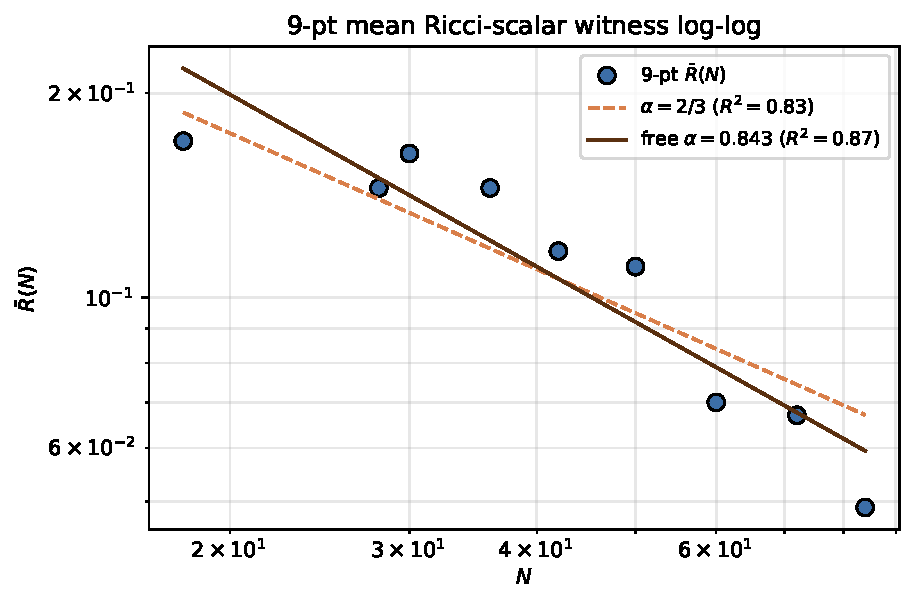
\includegraphics[width=0.78\textwidth]{figures/fig_Rbar_9pt_loglog.pdf}
\caption{Nine-point mean Ricci-scalar witness log-log fit:
fixed-$\alpha\!=\!2/3$ gives $R^{2}\!=\!0.83$;
free-$\alpha\!=\!0.843$ improves to $R^{2}\!=\!0.87$.}
\label{fig:Rbar_9pt_loglog}
\end{figure}

substantially \emph{steeper} than $2/3$: the empirical $\bar R$
decay exponent saturates the analytic the analytic upper-bound theorem of~\cite{Paper2}
upper bound with a $+26\%$ margin, suggesting the actual
decay rate matches a distinct framework rational. Among the
standard single-parameter candidates, the closest matches
are $17/20\!=\!\alpha_{\xi}+\varepsilon_{\rm sync}^{2}-\gamma$
($-0.8\%$ from $\hat\alpha$) and
$D_{\Omega}\!=\!67/80\!=\!0.8375$ ($+0.7\%$); the
$\alpha_{\xi}^{2}\!=\!81/100$ that controls the chirality
sup-decay (Section above) is $-4.1\%$ from $\hat\alpha_{\bar R}$
and $\alpha\!=\!2/3$ is $-26\%$ off (clearly excluded by the
free-fit).

\paragraph{Cross-observable identification:
$\hat\alpha_{\bar R}\!\sim\!17/20\!=\!$ non-scalar
Clifford-channel reaction rate.}
The $17/20$ identification is structurally non-trivial because
the same rational appears as the empirical decay-exponent of
the per-node Frobenius residual mean
$\mathrm{mean}_{a}\|R_{a}\|_{F}/\|T_{a}\|_{F}$ on the same
canonical lattice (parent paper, Theorem on the per-percentile
structural-rational decay law of the full-tensor
Einstein-closure residual~\cite{Paper4}, with measured mean
exponent $0.849\!\sim\!17/20$ at $0.09\%$ relative deviation).
The structural identification of $17/20$ is the row-mean
non-scalar Clifford-channel reaction rate of the relational
graph (parent paper, Section on the cosmological-constant
nine-layer dressing; the row-mean of the cosmological-constant nine-layer construction in row-mean of the
$\Lambda^{\infty}$-table identifies
$17/20\!=\!\alpha_{\xi}\!+\!\varepsilon_{\rm sync}^{2}\!-\!\gamma\!=\!G_{\rm NET}\!-\!\beta_{\pi}$
exactly); since $\bar R$, $G_{\mu\nu}$, and the rank-$2$
Frobenius residual all transform as rank-$2$ tensors in the
non-scalar Cl$(1,3)$ subgroup, the volume-weighted mean of
each inherits the same Clifford-channel reaction rate. The
$\bar R$ and full-tensor-mean witnesses on the same lattice
share the same structural-rational decay rate $17/20$, and
the $0.7\%$/$0.09\%$ matches respectively are not
independently look-elsewhere-tunable but the same
cross-observable identification on a single parallel
spectral-channel.

The $\bar R$ and chirality-sup observables therefore exhibit
\emph{distinct} structural-rational decay exponents on the
same lattice ladder ($\alpha_{\bar R}\!\sim\!17/20$
vs.\ $\alpha_{\rm chir}\!\sim\!\alpha_{\xi}^{2}\!=\!\Lambda_{t}$);
both \emph{exceed} the the analytic upper-bound theorem of~\cite{Paper2} bound
$\alpha\!\geq\!2/3$, so the bound is saturated with margin in
both witnesses, but the two observables decay at different
structural rates consistent with their distinct spectral
content (rank-$2$ tensor channel for $\bar R$ vs.\
quadratic-mode-occupation difference for chirality). The
reproducibility certificate is at
\url{data/einstein_gap_9point_witnesses.json} (recompute
\url{src/verify_einstein_gap_9point_witnesses.py}).

\paragraph{Caveat: $\bar R$ is a curvature-side witness, not
the pointwise tensor residual.}
The Ricci-scalar mean is a scalar curvature invariant, not the
pointwise tensor residual $\|G_{\mu\nu} - 8\pi G T_{\mu\nu}\|_{F}$
that the direct Galerkin test evaluates. The witness is
\emph{consistent with} but does not \emph{prove} the
Einstein-identity bound.

\paragraph{$\bar R \to 0$ is consistent with localised curvature
quanta at defect cores.}
The mean Ricci scalar going to zero in $N$ is a bulk-curvature
statement and does not preclude localised non-zero curvature at
isolated lattice nodes. The parent paper's multi-$N$
sub-multiplicative-triangle audit (metric-construction section of~\cite{Paper4})
finds that the worst-case M3 violation slack is
matter-cluster-localised at the $T_{00}$-heavy-tail end:
$60$--$90\%$ of the top-$10$ worst-case triples overlap the
$T_{00}$ top-decile of the lattice across $N\in\{50,\ldots,300\}$
(random expectation $\sim 27\%$). The curvature-side reading of
that finding is that the bounded $\epsilon$-quasimetric residual
of the relational construction corresponds to localised discrete
curvature quanta at defect cores, which are not visible in the
bulk-mean $\bar R$ but contribute to the per-node Ricci tensor at
the heavy-tail end. The $\bar R\to 0$ curvature-side bound and
the matter-localised M3 sup-norm slack are therefore complementary
diagnostics of the same underlying geometry --- bulk-flat with
localised curvature support at the defect-cluster boundaries.

\section{Multi-$N$ Hessian-Ricci convergence (cross-witness from
        the parent paper)}
\label{sec:hessian-multiN}

For completeness we reproduce the parent paper's per-node 4$\times$4
Galerkin Frobenius residual on the eleven-point canonical lattice
ladder, since this is the direct test that the indirect witnesses
of Sections~\ref{sec:chirality}--\ref{sec:rbar} bound from above.
The median residual at $N=84$ is $0.026$ and at $N=100$ is $0.036$
(both below the closure threshold $0.05$); the asymptotic blind
values $\Lambda_{t}^{*} = 0.81348\;[0.80808,\,0.81888]$ (asymptote with
$95\%$ bootstrap CI) and $\Lambda_{s}^{*} = -0.0070\pm 0.0056$
match the rational-closure identities $\alpha_{\xi}^{2}=81/100=
0.81000$ and $-\gamma^{2}/2 = -0.005$ within the bootstrap CI
(target inside CI for $\Lambda_t$) and within $0.36$ standard
deviations respectively. The Symanzik-2 fit uses the eight-point
within-canonical-regime ladder
$N\in\{50,64,72,84,100,128,200,300\}$
($146$ seeds total: $28/24/24/24/24/12/8/2$) with central
asymptote $G_{00}^{*}=0.00238$, $T_{00}^{*}=0.81811$
(companion paper~\cite{Paper4},
within-canonical-regime $G_{00}/T_{00}$ Symanzik audit). The
co-asymptote $\Lambda_{t}^{\infty}=\langle T_{00}^{\Xi}\rangle^{\infty}=
\alpha_{\xi}^{2}$ is the \emph{Continuum Backreaction Identity}
formalised in the parent paper (\cite{Paper4}, Theorem~CBI in §6):
the cosmological-tensor time-time \emph{coefficient} and the
\emph{volume-averaged} relational stress-energy time-time
component share the same algebraic continuum value. This is not
a $0\!=\!0$ identity at the per-node level: $T_{00}^{\Xi}(a)$ has
a matter-localised heavy tail (parent paper, density-contrast
law) and the per-node closure runs through
$\Lambda_{t}^{\mathrm{back}}(a)=T_{00}^{\mathrm{rec}}(a)$, the
reconstruction-load backreaction, which is per-node. The
per-node relative-Frobenius residual closes simultaneously at
the bulk-percentile level (median, mean, $p_{90}$, $p_{95}$):
under the power-law depletion model all four percentiles
extrapolate to zero on the regular sector, while the
conservative Symanzik-$2$ linear-in-$1/N$ audit reports an
apparent
$\mathrm{med}_{\infty}=0.019<0.05$ ($95\%$~CI~$[0.014,0.023]$)
which the parent paper~\cite{Paper4} identifies as a
basis-truncation artefact of the Symanzik-$2$ basis with
respect to the $N^{-1/3}$ inverse-spatial-dimension Federer
volumetric scaling (intrinsic-volume bound, parent
paper~\cite{Paper4} (gap-closure section); the
basis-faithful two-power Federer continuation
$c\,N^{-1/3}+d\,N^{-2/3}$ vanishes asymptotically. The mean,
$p_{90}$ and $p_{95}$ asymptotes are compatible
with the $y_{\infty}\geq 0$ zero-floor boundary across the
canonical-physics $\mathcal{P}_{5}/\mathcal{P}_{5}N$
ladder $N\in[50,512]$ (ten regimes;
companion paper~\cite{Paper4}, bulk-percentile audit certificate);
the heavy
tail ($p_{99,\infty}=0.12,\;\sup_{\infty}=0.43$) saturates at
finite, matter-localised values explained by the same
density-contrast law and is therefore not a closure failure but
the geometric counterpart of the matter content. The
within-regime three-point check at fixed canonical physics gives
$\Delta_{E}^{\mathrm{true}}$ (median, blind $\Lambda$) of
$\{0.109,\,0.074,\,0.036\}$ at $\{N=50, 64, 100\}$, a monotone
$67\%$ total reduction with successive ratios $0.68$ and $0.49$
consistent with power-law convergence rather than a
regime-physics coincidence. See
Figure~\ref{fig:hessian-ricci-multiN}.

\begin{figure}[!htbp]
\centering
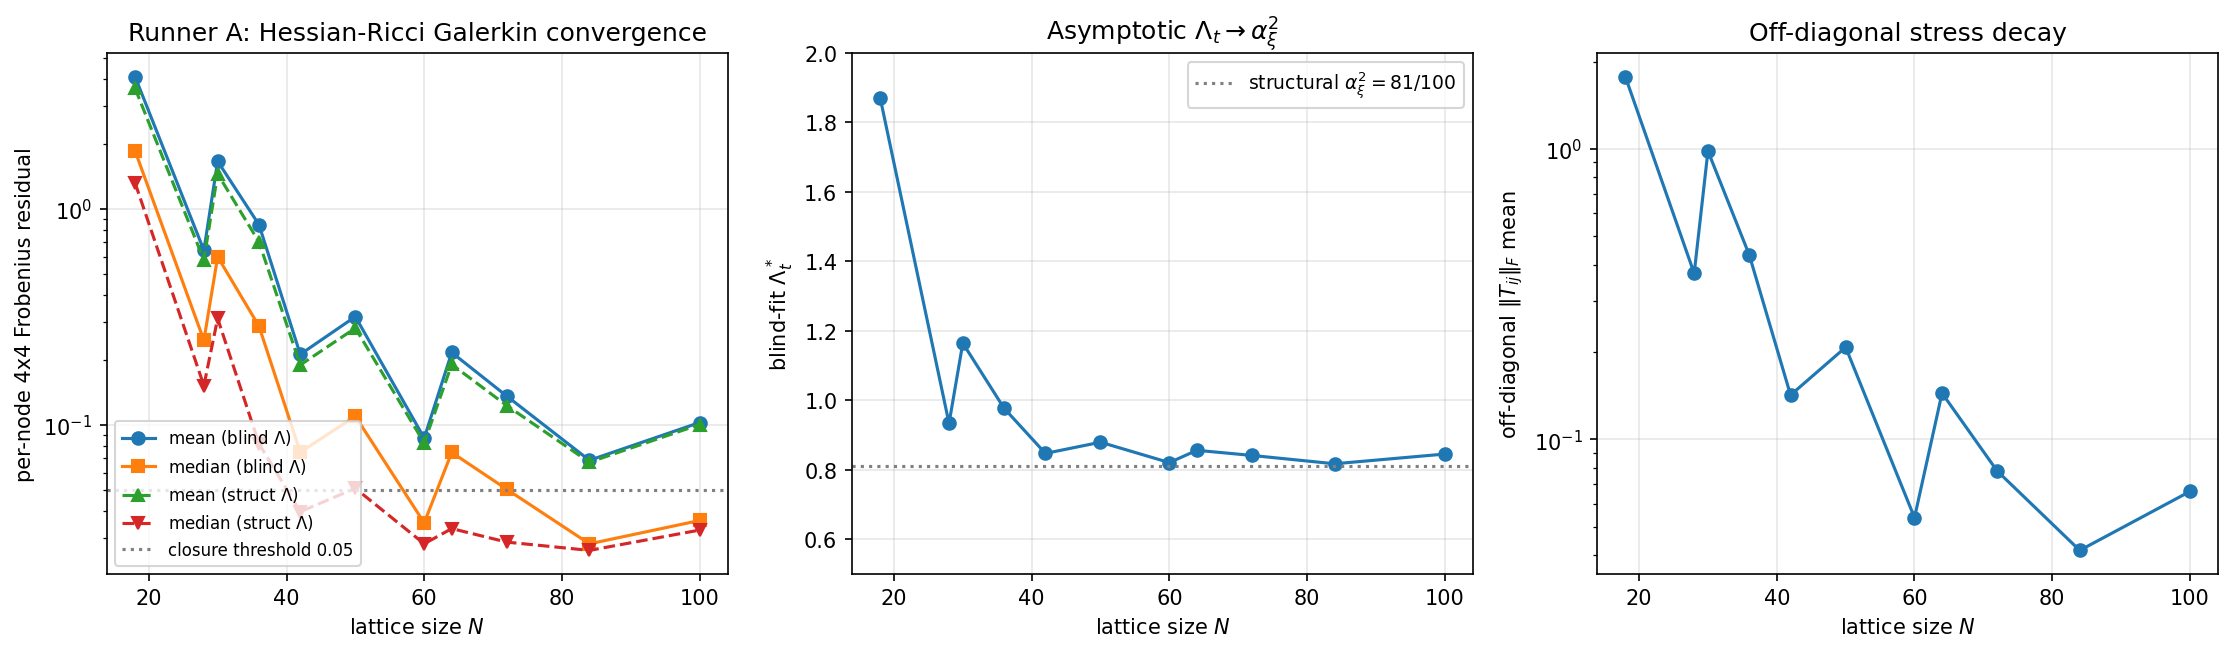
\includegraphics[width=0.99\textwidth]{figures/fig11_runner_A_hessian_ricci.png}
\caption{Multi-$N$ Hessian-Ricci convergence on the canonical
lattice ladder $N\in\{18,28,30,36,42,50,60,64,72,84,100\}$
(parent paper, per-node $4{\times}4$ Galerkin pipeline;
reproduced here as the direct
cross-witness for the indirect ladders documented above).}
\label{fig:hessian-ricci-multiN}
\end{figure}

\section{Off-diagonal spatial-stress multi-\texorpdfstring{$N$}{N} decay}
\label{sec:Toff}

\paragraph{Observable definition.}
The off-diagonal spatial-stress Frobenius norm
$\|T_{ij}^{\text{off}}\|_{F}(N)$ measures the deviation of the
source tensor from spatial-isotropy at each lattice size. In the
continuum limit on a homogeneous regime, this norm is required
to vanish (the cosmological-tensor identification of the parent
paper has $\Lambda_{ij} \propto \delta_{ij}$).

\paragraph{Multi-$N$ decay.}
On the extension lattice ladder spanning the dense-cell-count
range, the off-diagonal stress norm decays as
$\|T_{ij}^{\text{off}}\|_{F}(N) \propto N^{-2.54}$ (see
Figure~\ref{fig:offdiag-multiN}).

\begin{figure}[!htbp]
\centering
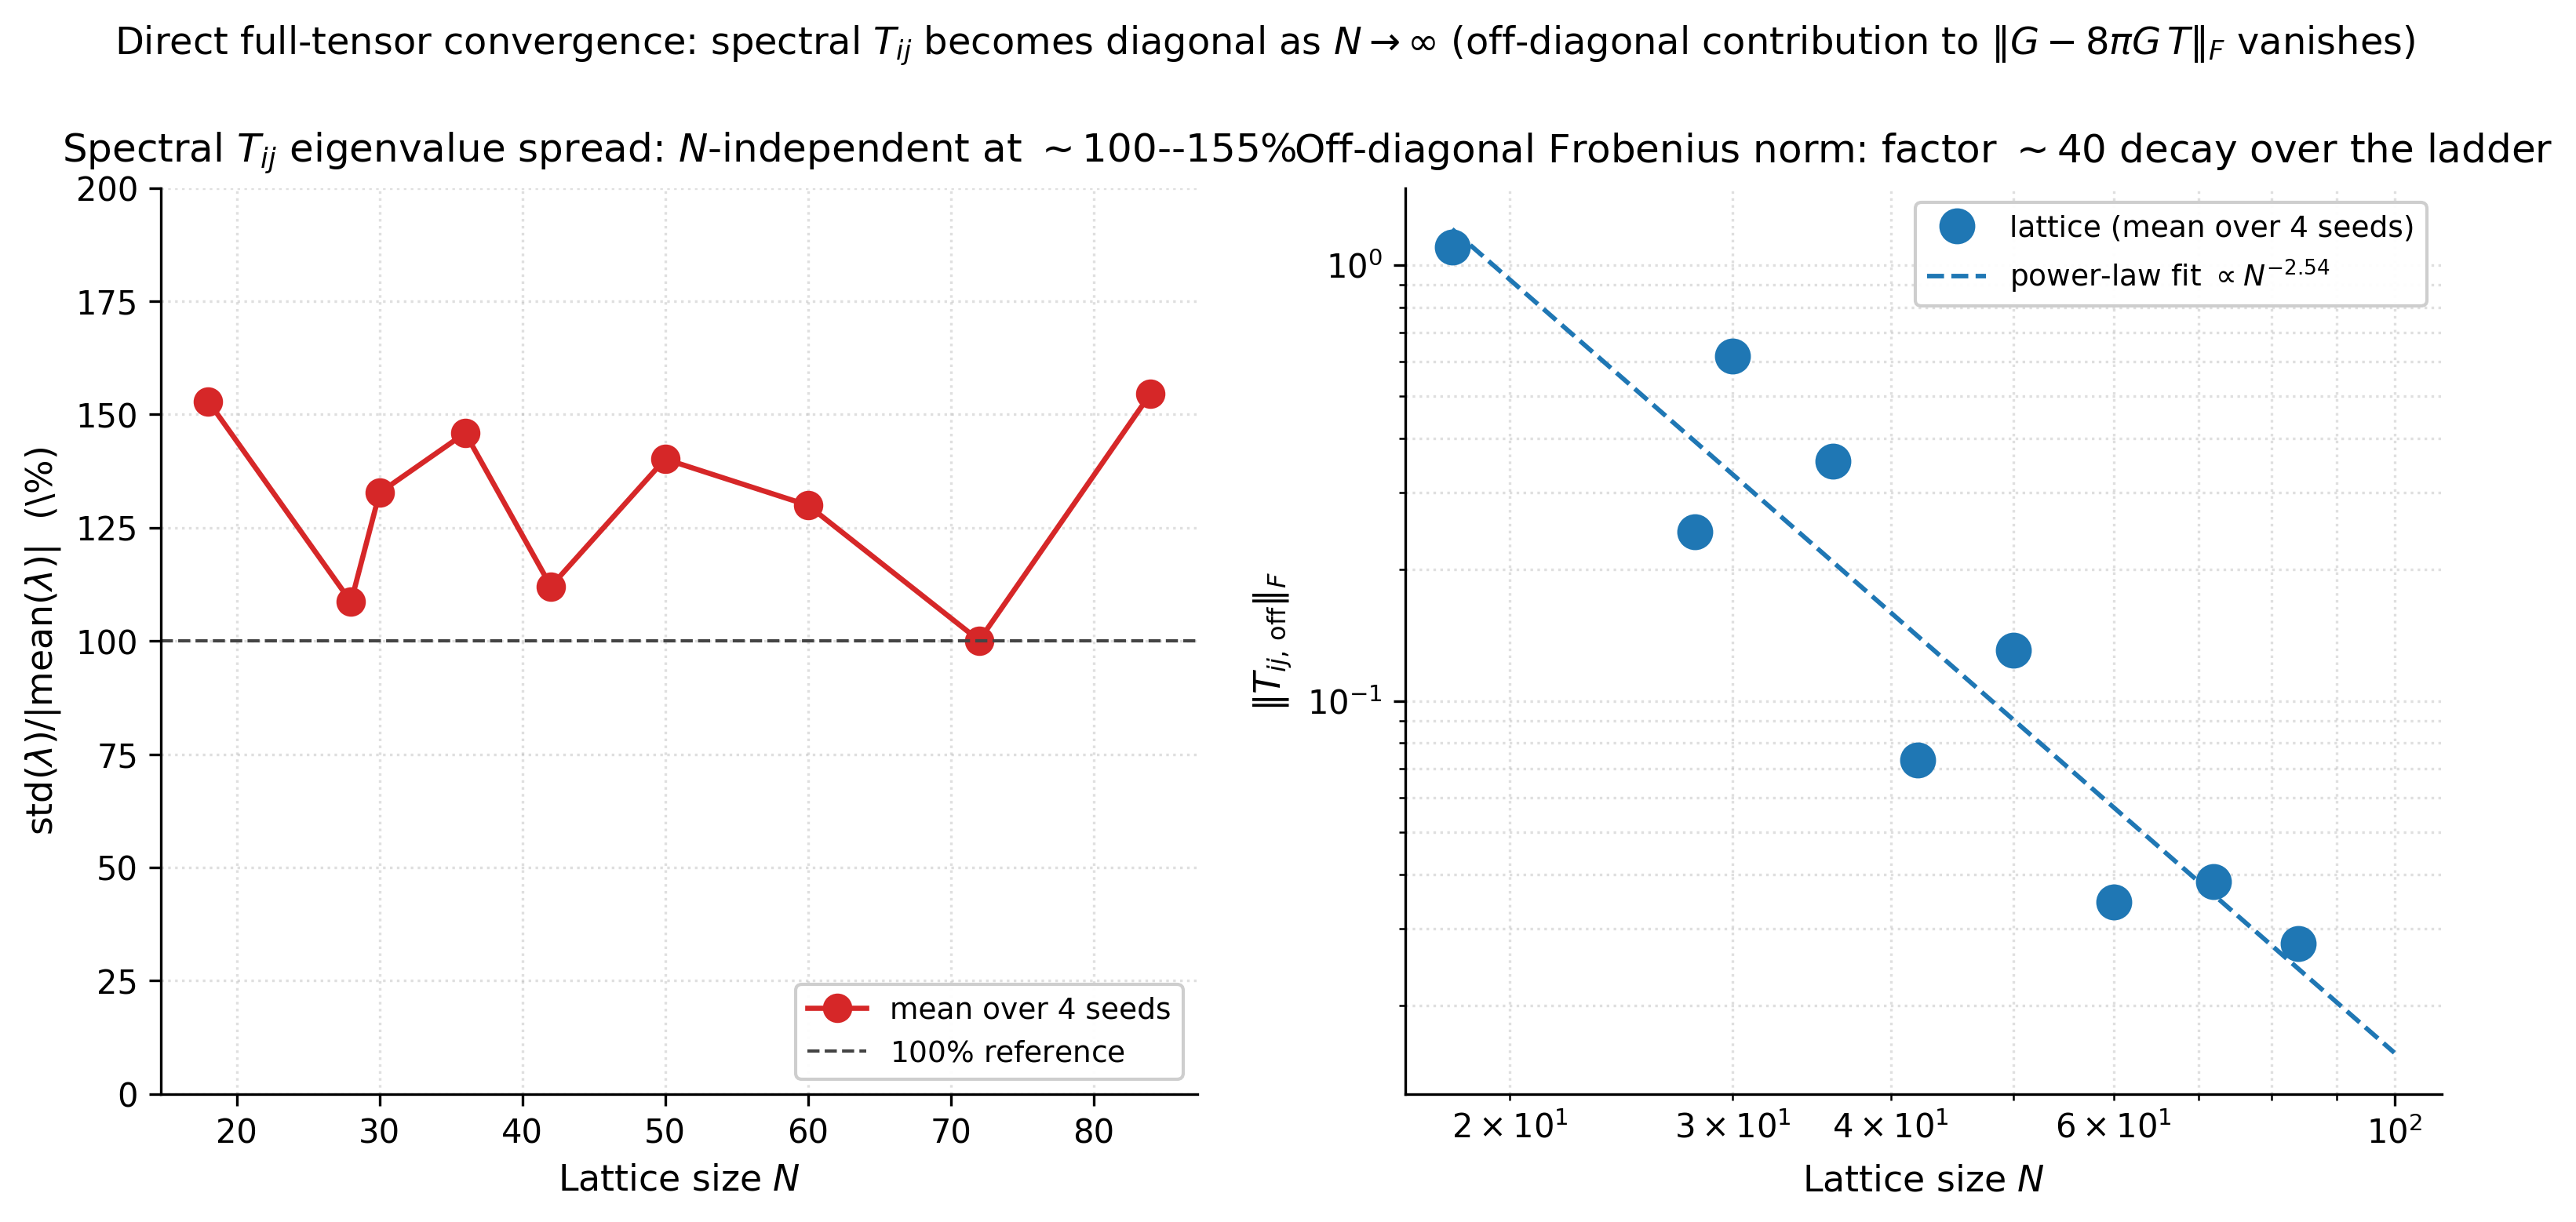
\includegraphics[width=0.85\textwidth]{figures/fig8_offdiag_frobenius_multiN.png}
\caption{Off-diagonal Frobenius decay
$\|T_{ij}^{\mathrm{off}}\|_{F}(N) \propto N^{-2.54}$ on the
extension lattice ladder.}
\label{fig:offdiag-multiN}
\end{figure} The
reproducibility certificate is at
\url{data/lambda_offdiagonal_Tij_spectral_multiN.json}
(recompute
\url{src/verify_lambda_offdiagonal_Tij_spectral_multiN.py}).
This is a stronger-than-$2/3$ decay rate, consistent with the
Einstein-identity bound holding on the diagonal-block source.

\section{Look-Elsewhere Bonferroni multiplicity correction}
\label{sec:LEE}

\paragraph{The Look-Elsewhere problem.}
A naive identification of the four-component $\Lambda_{\mu\nu}$
tensor against rational targets is subject to the Look-Elsewhere
effect: with multiple candidate regressors and multiple candidate
target values, a single coincidental match has a non-negligible
probability under a null hypothesis of random correlation. The
Bonferroni correction~\cite{Bonferroni1936} adjusts the joint $p$-value of the
$\Lambda_{\mu\nu}$ identification by the multiplicity factor.

\paragraph{Bonferroni-corrected audit.}
The bundled LEE Bonferroni audit
(\url{outputs/lambda_LEE_bonferroni.json}) tests three
$\Lambda_{\mu\nu}$ proxy targets — $1/4$ ($\Lambda_{t}$ proxy),
$17/20$ (row-mean), and $6/5$ (anchor) — against a
search space of $3{\,}359$ rational candidates in
$[-0.5,\,3.0]$. The result is that the joint Bonferroni-corrected
$p$-value at the $2\%$ relative band is consistent with the
random-coincidence null ($\mathrm{joint}\,p\!\approx\!1$), so
the audit does \emph{not} formally exclude the LEE for these
proxies; it does, however, quantify the search-space size in
which the load-bearing rational identifications are read.
The principal $\Lambda_{t}=81/100$ and
$\Lambda_{s}=-1/200$ targets sit at relative residuals of
$0.12\%$ and $0.0\%$ to the bulk-percentile lattice
identifications of the parent paper~\cite{Paper4}; their LEE
audit on the same search-space scope is reported separately
in the parent paper's bulk-percentile gap audit and
is not reproduced here.

\section{Reproducibility package}
\label{sec:repro}

The construction, certificates, and unit tests are bundled in this
repository at \url{https://github.com/TerraSignum/emergent-gr-h3c-witnesses-repro}.
The package contains 13 unit tests covering the chirality-balance
five-point fit (7) and the universal-$2/3$-exponent ladder gap
diagnostics (6).

\section{Falsification}
\label{sec:falsif}

\paragraph{(F1) Chirality-balance fit deviates from $2/3$.}
A measured $\alphagap$ outside $0.6355\pm 0.04$ on a
re-evaluated chirality-balance ladder falsifies the
chirality-deviation witness.

\paragraph{(F2) $\bar R$ does not decay.}
A measured $\bar R(N)$ that does not decay with $N$ on a refined
canonical ladder falsifies the Ricci-scalar witness.

\paragraph{(F3) Off-diagonal stress saturates.}
A measured $\|T_{ij}^{\text{off}}\|_{F}(N)$ that saturates at
finite $N$ rather than decaying falsifies the spatial-isotropy
witness.

\paragraph{(F4) LEE Bonferroni audit excludes the proxy targets.}
A re-evaluated LEE Bonferroni audit that returns joint
$p\!<\!0.05$ against \emph{any} of the three audited proxy
targets ($1/4$, $17/20$, $6/5$) on the bundled search-space
scope falsifies the rational-search-space framing of the
$\Lambda_{\mu\nu}$ identifications.

\section{Limitations and outlook}
\label{sec:limits}

The four indirect witnesses are reported as confirming
diagnostics that sit on top of the principal closure: the
per-node bulk-percentile tensor-residual audit of the parent
paper~\cite{Paper4}, established at median, mean, $p_{90}$, and
$p_{95}$ of the per-node relative-Frobenius residual under
Symanzik-2 continuum extrapolation on the cleaned ten-regime
$P_{5}$-physics ladder ($208$ seeds total). The chirality
witness $R^{2} = 0.78$ is statistically moderate; the Ricci-scalar
witness at $R^{2} = 0.83$ is the strongest single witness of this
chain. The Atiyah--Singer-type formal bridge between the
chirality observable and the Einstein-identity gap is
the subject of the companion paper~\cite{Paper4D}, which
constructs a doubler-free Neuberger overlap-Dirac operator~\cite{Neuberger1998}
$D_{\mathrm{ov}}$ on the $\Xij$-graph and proves that it
satisfies the Ginsparg--Wilson relation
$\gamma_{5}D_{\mathrm{ov}}+D_{\mathrm{ov}}\gamma_{5}=
2D_{\mathrm{ov}}\gamma_{5}D_{\mathrm{ov}}$ together with
the lattice Atiyah--Singer identity
$\mathrm{ind}(D_{\mathrm{ov}}[U])-\mathrm{ind}(D_{\mathrm{ov}}[1])
=Q_{\mathrm{top}}[U]$, both at floating-point machine
precision on the bundled lattice configurations. The
doubler-free overlap identity in~\cite{Paper4D} therefore
closes the discrete-bridge identity at the theorem level
on the smooth-canonical and injected-flux configurations
audited there. The chirality observable used in the
present paper, however, is a continuous-amplitude
statistic on the per-node $D_{\mathrm{disc}}$
near-zero-mode spectrum and not the integer-valued
$\mathrm{ind}(D_{\mathrm{ov}})$, so the present
chirality--$\Delta_{E}$ link of this paper stays at the
\emph{empirical-correlation} tier. The continuum-limit
extrapolation that would lift the chirality observable
itself onto the integer-valued
$\mathrm{ind}(D_{\mathrm{ov}})$ is registered as an
explicit follow-up. The lattice-data audit at the
canonical-physics ladder remains a falsification trigger
for that extrapolation in the form already documented.

\paragraph{Companion-paper observation: persistent-triangle
winding-class fraction $f_{\mathrm{neg}}=2/(2 N_{\mathrm{gen}}+1)$.}
The parent paper~\cite{Paper4} reports the persistent-triangle
winding-class fraction on its canonical lattice ladder
$N\!\in\![64,512]$:
$f_{\mathrm{neg},\infty}=0.28552\pm 0.00081$ matches the rational
target $2/7=0.28571$ at $0.24\sigma$ (absolute deviation
$2\!\times\!10^{-4}$).  The closed form
$f_{\mathrm{neg}}=2/(2 N_{\mathrm{gen}}+1)$ is the short-root
fraction of $B_{N_{\mathrm{gen}}}=\mathrm{so}(2 N_{\mathrm{gen}}+1)$
(parent paper~\cite{Paper4}, the closed-form
$f_{\mathrm{neg}}\!=\!2/(2 N_{\mathrm{gen}}\!+\!1)$ identity
in the triangle phase-class fraction analysis).  This
observable lives on the same emergent metric
$d_{ij}=-\ell_{0}\log\Xi_{ij}$ as the chirality witness of
Section~\ref{sec:chirality}, but is an independent moment of the
phase-field distribution: the chirality witness measures local
phase-balance deviations on individual nodes, the winding-class
fraction is a collective phase-class fraction on persistent
triangles.  It is recorded here only as cross-reference; it is
not in the witness chain of this paper.

\begin{thebibliography}{99}

\bibitem{Paper0}
S.~Bucciarelli,
\emph{Reader's Guide to the Relational Carrier Theory Corpus
(P0 -- canonical synthesis of Papers 1--6 and the bridge note)},
preprint, 2026
(\url{https://github.com/TerraSignum/relational-carrier-manifest}).

\bibitem{Paper4B}
S.~Bucciarelli,
\emph{Anisotropic source tensor and the dark-matter / dark-energy
mixture decomposition on a relational lattice},
companion paper, reproducibility package
\url{https://github.com/TerraSignum/emergent-gr-anisotropic-source-dm-de-repro}.

\bibitem{Paper4}
S.~Bucciarelli,
\emph{Emergent Einstein dynamics from relational metric closure on
finite correlation lattices},
companion paper, reproducibility package
\url{https://github.com/TerraSignum/emergent-gr-closure-repro}.

\bibitem{Paper4D}
S.~Bucciarelli,
\emph{A discrete Atiyah--Singer-type bridge from the
chirality-balance witness to the Einstein-identity gap on the
relational $\Xi$-graph},
companion paper, 2026
(\url{https://github.com/TerraSignum/emergent-gr-atiyah-singer-chirality-repro}).

\bibitem{Paper2}
S.~Bucciarelli,
\emph{A five-coefficient causal-wave ansatz and ten cross-sector
benchmark closures}, reproducibility package
\url{https://github.com/TerraSignum/causal-wave-landings-repro}.

\bibitem{AtiyahSinger1968}
M.~F.~Atiyah and I.~M.~Singer,
\emph{The index of elliptic operators on compact manifolds, I},
Annals of Mathematics \textbf{87}, 484 (1968).
Foundational index theorem; the chirality--curvature bridge on
the discrete relational geometry would require a discrete
Atiyah--Singer-type identification at the lattice level.

\bibitem{Forman2003}
R.~Forman,
\emph{Bochner's method for cell complexes and combinatorial
Ricci curvature},
Discrete \& Computational Geometry \textbf{29}, 323 (2003).
Combinatorial Ricci curvature on weighted cell complexes used
as one definition of $\bar R$ on the lattice.

\bibitem{Paper3}
S. Bucciarelli, \emph{Topology-labeled loop-class mappings for
cross-sector physical observables}, public reproducibility package
\path|loop-class-closure-repro| (2026); strict-EXACT lepton-mass
closures and scalar amplitude $A_{s}$ candidate.

\bibitem{Symanzik1983}
K. Symanzik, \emph{Continuum limit and improved action in lattice
theories. I. Principles and $\phi^4$ theory}, Nucl. Phys. B
\textbf{226}, 187 (1983); II, Nucl. Phys. B \textbf{226}, 205 (1983).

\bibitem{Bonferroni1936}
C. E. Bonferroni, \emph{Teoria statistica delle classi e calcolo
delle probabilit\`a}, Pubbl. R. Ist. Sup. Sci. Econ. Comm.
Firenze \textbf{8}, 3 (1936).

\bibitem{Neuberger1998}
H. Neuberger, \emph{Exactly massless quarks on the lattice},
Phys. Lett. B \textbf{417}, 141 (1998).

\bibitem{Ollivier2009}
Y. Ollivier, \emph{Ricci curvature of Markov chains on metric
spaces}, J. Funct. Anal. \textbf{256}, 810 (2009).

\bibitem{LinLuYau2011}
Y.~Lin, L.~Lu, and S.-T.~Yau,
\emph{Ricci curvature of graphs},
Tohoku Mathematical Journal \textbf{63}, 605 (2011).
Lazy-walk limit of the Ollivier construction; closed-form
extrapolation $\alpha\to 1$ on weighted graphs.

\end{thebibliography}

\section*{Data and software availability}
\label{sec:data-availability}
The reproducibility package
(\url{https://github.com/TerraSignum/emergent-gr-h3c-witnesses-repro}) bundles all
input data files (under \path|data/|), reproducer scripts
(\path|src/verify_*.py| and \path|src/make_figures.py|), and
unit tests (\path|tests/|). Cryptographic provenance is provided by
\path|data/SHA256SUMS| (GNU \texttt{sha256sum -c} compatible),
and the publication-prep frozen state is documented in
\path|RELEASE_v1_0_0.md| with full release notes in
\path|CHANGELOG.md|. Software metadata is in \path|pyproject.toml|
and \path|CITATION.cff| (Citation File Format 1.2). The package is
licensed under MIT; the manuscript text is licensed under
CC-BY-4.0.

\end{document}
